\section{Numerical experiments}
\label{sec:experiments}

We compare CCSGD with naive SGD, second- and fourth-order Taylor
correction, quadratic SIMEX, the deterministic Woolsey--Huang Eq.~(5)
correction, and regression calibration. Responses are noise-free; Gaussian
measurement noise is added only to the inputs. Appendix~\ref{app:experiment_details}
specifies the baseline updates and population-bias calculations.

\subsection{Nonlinear-feature regression}
We use
\[
\psi(z)=(\sin z,\cos(0.7z),z^2)^\top,\qquad
Y=\theta_{\rm true}^\top\psi(Z),\qquad
\ell(\theta;z,y)=\tfrac12(\theta^\top\psi(z)-y)^2,
\]
where $\theta_{\rm true}=(0.8,-0.6,0.2)^\top$ and
$Z\sim0.8N(-0.5,0.8^2)+0.2N(2,0.8^2)$.
The algorithms observe $(W,Y)$ with $W=Z+U$ and
$U\sim N(0,1.2^2)$ independent of $Z$.
CCSGD evaluates the full score at $W+iV$, with an independent
$V\sim N(0,1.2^2)$ at each update, using complex arithmetic.
All runs use fresh latent samples and fresh measurement noise.
The objective is quadratic and strongly convex in $\theta$, despite its
nonlinear dependence on $z$. Appendix~\ref{app:regression} verifies the
relative variance bound directly and gives the $O(t^{-1})$ MSE rate.
Figure~\ref{fig:nonlinear_regression_mse} shows a fitted slope of $-0.978$,
consistent with this rate, while the specified approximate updates approach
nonzero population biases.

\begin{figure}[H]
\centering
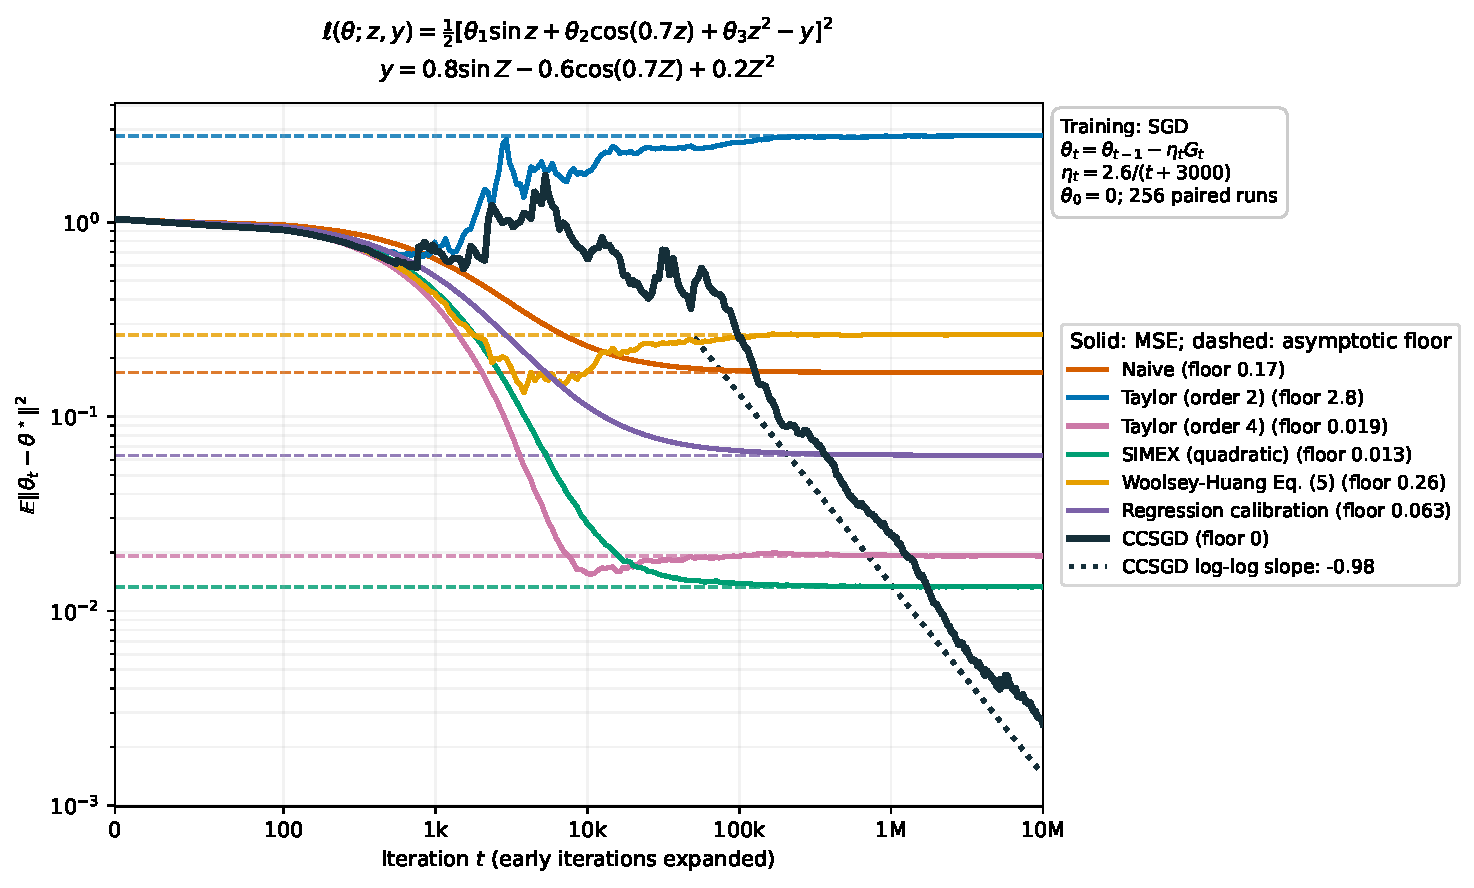
\includegraphics[width=\textwidth]{figure_regression.pdf}
\caption{Parameter MSE averaged over 256 paired runs, starting at
$\theta_0=0$ with $\eta_t=2.6/(t+3000)$.
Dashed lines show the calculated asymptotic squared biases of the specified
baseline updates. Quadratic SIMEX extrapolates three separately optimized
parameter trajectories; its additional Gaussian noise is integrated exactly.
The Woolsey--Huang baseline uses their deterministic Eq.~(5) correction.
The dotted CCSGD guide has fitted log--log slope $-0.978$ over
$5\times10^4\le t\le10^7$.}
\label{fig:nonlinear_regression_mse}
\end{figure}

\subsection{Neural-network regression}
We generate noise-free responses from
\[
Z\sim\operatorname{Unif}[-2,2],\qquad
Y=f_0(Z)=e^{-Z^2}\sin(3Z)+0.3Z^2,
\]
and fit a single-hidden-layer network
\[
h_\theta(z)=c+\sum_{j=1}^{32}a_j\sin(b_jz+d_j),\qquad
\ell(\theta;z,y)=\tfrac12(h_\theta(z)-y)^2,
\]
training all 97 parameters. For each fixed finite parameter vector, the
score is entire and has at most exponential growth in the input; its
Gaussian complex correction is therefore unbiased with finite second
moment. The exponential rate can depend on the input weights; neither
a parameter-independent exponent nor the amplitude control in
\eqref{eq:amplitude_control} is established for this network. Its training
curves are therefore empirical and do not invoke the nonconvex theorem.

We use 8,192 latent training pairs and 4,096 independent clean prediction
pairs, with no validation set. At every minibatch presentation, we generate
fresh $U\sim N(0,0.3^2)$ and observe $W=Z+U$; all methods share these
observations, minibatch indices, and initialization. CCSGD independently
samples $V\sim N(0,0.3^2)$ and computes
\[
\operatorname{Re}\left[(h_\theta(W+iV)-Y)
\nabla_\theta h_\theta(W+iV)\right]
\]
using complex arithmetic and the analytic squared loss, without complex
conjugation. Training uses minibatches of size 128 and
$\eta_t=0.01(1+t/2000)^{-0.6}$.

We compare naive SGD, Taylor corrections of orders two and four,
quadratic SIMEX, the Woolsey--Huang Eq.~(5) correction, and regression
calibration. Taylor corrections differentiate the full score with respect
to its input, holding the response fixed. SIMEX trains separate networks
at additional noise levels $\lambda=0,1,2$ and extrapolates predictions as
$3h^{(0)}-3h^{(1)}+h^{(2)}$. Regression calibration uses the exact
$\mathbb E[Z\mid W]$ under the specified uniform latent distribution.
The prediction set is used only to report
$n_{\rm pred}^{-1}\sum_i(h_{\theta_t}(Z_i)-Y_i)^2$.

\begin{figure}[H]
\centering
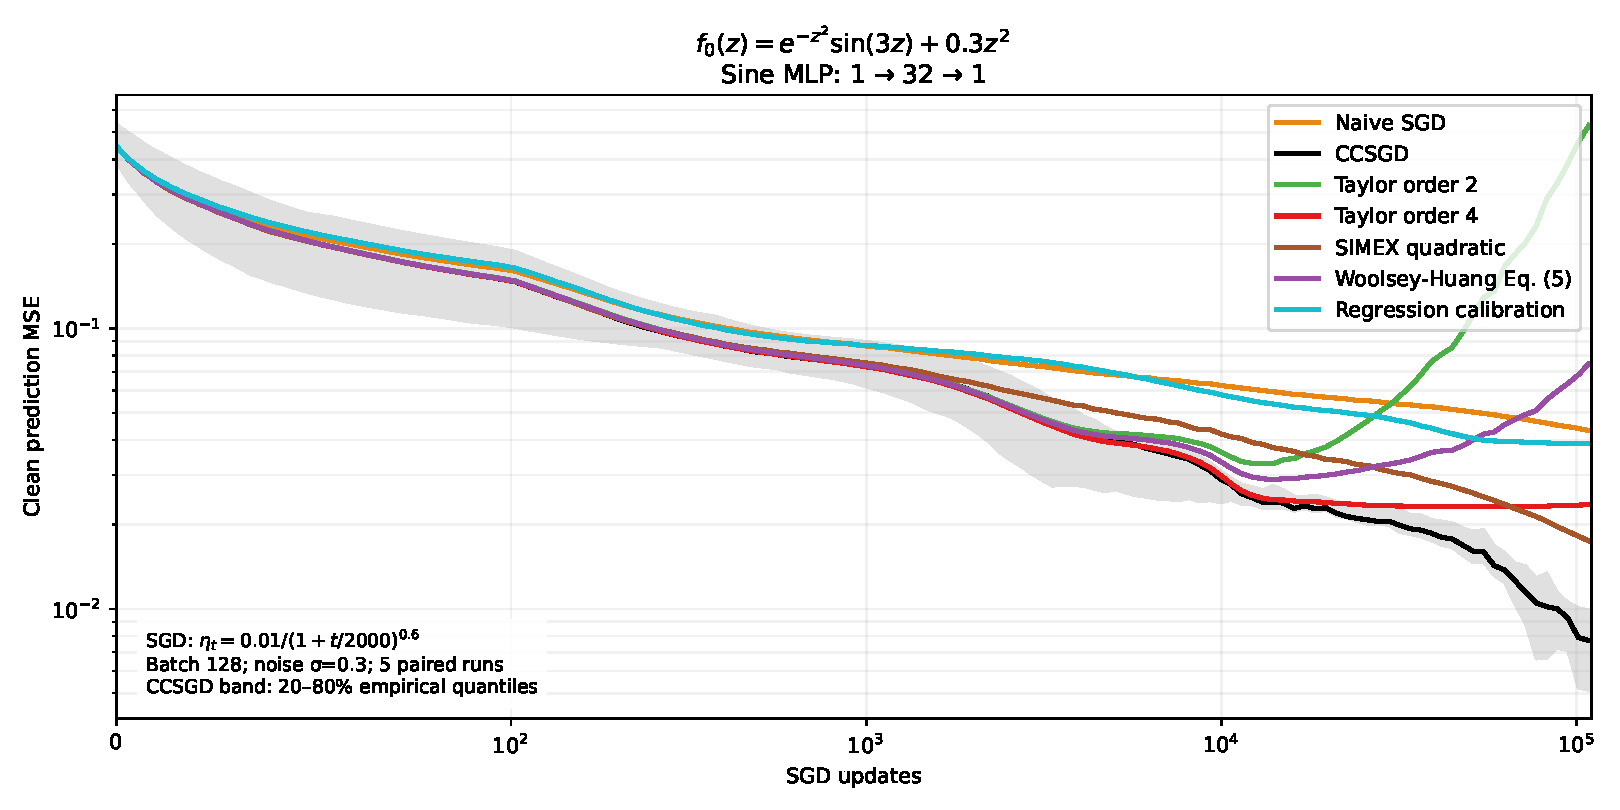
\includegraphics[width=\textwidth]{figure_neural_network.pdf}
\caption{Clean-input prediction MSE averaged over five paired runs.
The shaded CCSGD band gives empirical 20--80\% quantiles.
Training runs for 200,000 updates; the figure displays the trajectory
through $1.1\times10^5$ updates. CCSGD attains lower mean prediction error
than the specified baselines near the displayed endpoint.}
\label{fig:neural_network_mse}
\end{figure}

This experiment targets the clean empirical training objective conditional
on the latent training set. Fresh measurement noise preserves conditional
unbiasedness for that objective; it does not remove finite-sample or
approximation error on the independent prediction set. The methods'
ordering changes during training: at 200,000 updates, mean prediction
MSE is $0.0142$ for CCSGD and $0.0125$ for SIMEX. These results illustrate
finite-time behavior without asserting a zero prediction-error limit.
